%% Copyright (C) 2007 Google Inc.
%%	
%% Licensed under the Apache License, Version 2.0 (the "License");
%% you may not use this file except in compliance with the License.
%% You may obtain a copy of the License at
%%
%% http://www.apache.org/licenses/LICENSE-2.0
%%
%% Unless required by applicable law or agreed to in writing, software
%% distributed under the License is distributed on an "AS IS" BASIS,
%% WITHOUT WARRANTIES OR CONDITIONS OF ANY KIND, either express or implied.
%% See the License for the specific language governing permissions and
%% limitations under the License.
%% ...........................................................................

%\documentclass[letterpaper,onecolumn,10pt]{article}
\documentclass[letterpaper,twocolumn,10pt]{article}

\usepackage{graphics}
\usepackage{hyperref}
\usepackage{alltt}
\usepackage{color}
\newcommand{\myurl}[1]{{\href{http://#1}{\texttt{#1}}}}
\newcommand{\myurlt}[2]{{\href{http://#1~#2}{\tt #1{\twiddle}#2}}}
\newcommand{\myurlh}[3]{{\href{http://#1#3}{\tt #1#2#3}}}

\definecolor{darkgray}{gray}{0.2}
\newcommand{\rem}[1]{{\textcolor{darkgray}{{\rm #1}}}}
\newcommand{\q}[1]{{\includegraphics{#1}}}
\newcommand{\qq}[2]{{\includegraphics{#1}}$\rightarrow${\includegraphics{#2}}}

% Add functionality for TODOs
% definitions.tex -- 
% Author          : Jasvir Nagra <jas@cs.auckland.ac.nz>
% Created On      : Tue Jun  3 12:58:52 2008
% Last Modified   : <08/06/03 14:06:12 jasvir>
% Description     : Additional helpful macros for formatting caja paper
% Keywords        : caja format latex
% Purpose         : Caja

% --------------------------------------------------------------------
%                              TODO list
% --------------------------------------------------------------------

\makeatletter

% Usage: \TODO{username}{Make this section clearer}
\newcommand{\TODO}[2]{
    \addcontentsline{todolist}{todo}{\protect{{\bf #1}:~#2}}
    \textcolor{red}{{\bf #1}: {\sf #2}}
}
\newcommand\l@todo[2]{\par \noindent Page~#2~\protect{\mbox{#1}}} 
\newcommand \listoftodos{\section*{TODO List} \@starttoc{todolist}}\makeatother

\endinput

% Emacs bunkum
% Local Variables:
% mode: latex
% time-stamp-start: "Last Modified[ \t]*:[ 	]+\\\\?[\"<]+"
% time-stamp-end:   "\\\\?[\">]"
% End:

%% Literal code-like strings in normal text.
\newcommand{\code}[1]{{\tt {#1}}}              % code

%don't want date printed
% \date{}

\sloppypar

\title{Caja\\
Safe active content in sanitized JavaScript}
\author{
        {\rm Mark S. Miller}
        \and 
        {\rm Mike Samuel}
        \and 
        {\rm Ben Laurie}
        \and 
        {\rm Ihab Awad}
        \and 
        {\rm Mike Stay}}


\begin{document}

\listoftodos

\maketitle

% Use the following at camera-ready time to suppress page numbers.
% Comment it out when you first submit the paper for review.
% \thispagestyle{empty}
% \pagestyle{empty}

\abstract

Using Caja, web apps can safely allow scripts in third party content.

The computer industry has only one significant success enabling documents to 
carry active content safely: scripts in web pages. Normal users regularly 
browse untrusted sites with JavaScript turned on. Modulo browser bugs and 
phishing, they mostly remain safe. But even though web apps build on this 
success, they fail to provide its power. Web apps generally remove scripts 
from third party content, reducing content to passive data. Examples include 
webmail, groups, blogs, chat, docs and spreadsheets, wikis, and more; whether 
from Google, Yahoo, Microsoft, HP, Wikipedia, or others.

Were scripts in an object-capability language, web apps could provide active 
content safely, simply, and flexibly. Surprisingly, this is possible within 
existing web standards. Caja represents our discovery that a subset of 
JavaScript is an object-capability language.

\ \\

\section{Introduction}

An \emph{object-capability language} is essentially a memory-safe object 
language with encapsulation, with additional restrictions that \emph{protect 
the outside world from the objects}.\footnote{
%
Thanks to Mark Lillibridge for this formulation.
%
}  In a memory-safe object language such as JavaScript, object A can only invoke 
object B if A has a reference to B. If A already has references to B and C, A 
can invoke B passing C as an argument, giving B access to C. Memory-safe 
object languages with encapsulation, such as Java, \emph{protect objects from 
the outside world}. The clients of an encapsulated object can make requests 
using its public interface, but how an object reacts to a request is up to 
the object. An encapsulated object can ensure that the only way to invoke its 
code or change its state is through its public interface.

In an object-capability language, an object can only cause effects outside 
itself by using the references it holds to other objects. Objects have no 
powerful references by default, and are granted new references only by normal 
message passing rules. Object references thereby become the sole 
representation of rights to affect the world, and normal message passing 
(method invocation) is 
the only rights transfer mechanism. An object can be denied authority simply 
by not giving it those references which would provide that authority.

The browser sandbox already mostly protects the world outside the browser 
from scripts running on web pages. A great virtue of JavaScript is that many 
people successfully program in it casually, without first learning the 
language in any depth. Caja\footnote{
%
\emph{Caja}, pronounced ``KA-hah'', is Spanish for ``box''. With Caja, 
\textbf{c}apabilities \textbf{a}ttenuate \textbf{J}avaScript 
\textbf{a}uthority.
%
} is a subset of JavaScript we designed to make as little impact as 
possible on regular JavaScript programming, while still providing 
object-capability security.  The subset is enforced by a static verifier
and the insertion of runtime checks into the code.  In this section, we provide a brief inaccurate 
overview of the differences between Caja and JavaScript suitable for the 
casual JavaScript programmer. The rest of this document then accurately goes 
into more depth.

\begin{figure}[t!]
\begin{alltt}
function F(x)\ \{ this.x_ = x; \}
F.prototype.getX = function()\ \{
  return this.x_;
\};
F.make = function(x)\ \{
  return new F(x);
\};
function test()\ \{
  return new F(3).getX() === 3;
\}
\end{alltt}

\caption[Caja Functions]{Caja Functions. \code{F} is a \emph{constructor}. It 
can only be initialized and used with \code{new} and \code{instanceof}. 
The function \code{F.prototype.getX} is a \emph{method}. It can only be called as a 
method. \code{F.make} and \code{test} are \emph{simple functions}. They are
not restricted. \\ } \hrule
\label{fig:func-obj}
\end{figure}

\begin{description}

  \item[Forbidden names.] In Firefox, access to the ``\code{\_\_proto\_\_}'' 
  property of an object would grant the authority to create more objects
  like it, which violates the principle of least authority.  Therefore, 
  Caja rejects all names ending with ``\_\_'' (double 
  underscore). This also gives the Caja implementation a place to store its 
  bookkeeping information where it is invisible to the Caja programmer.
 
  \item[Frozen objects.] In JavaScript, all objects are mutable, so passing
  the same reference to two objects automatically grants them the authority
  to communicate, which is undesirable.  
  Therefore, Caja adds the ability to \emph{freeze} an 
  object. If an object is frozen, an attempt to set, add, or 
  delete its properties will throw an exception instead. Functions and 
  prototypes are implicitly frozen. In addition, the Caja programmer can 
  explicitly freeze objects to prevent their direct modification. All objects 
  in the default global environment are \emph{immutable}, or transitively 
  frozen.
  
  \item[No shared global environment.] Caja code is compiled into units of
  isolation called \emph{modules}; in practice, these are JavaScript functions.  
  A \emph{container} loads the modules and grants them authority by means of 
  references passed as arguments to the module functions.  These arguments
  are called \emph{imports}.
  
  A module that displays the local 
  weather on a webpage should not be able \emph{a priori} to communicate 
  with a module that has access to your bank account. Therefore, each 
  module has its own global environment which inherits 
  from the default global environment, isolating them from each other.
  On the other hand, a container can allow two chosen modules to communicate
  by passing a reference to a common mutable object to each module.

  \item[Protected names.] The state of an object that is not part of its 
  public interface should not be read or changed by the outside world.  
  Javascript supports private variables via closures, but this pattern 
  incurs a large memory overhead.  Also, using this as the sole 
  encapsulation mechanism for object patterns conflicts with existing 
  JavaScript programming practice.  Therefore, Caja enforces the
  convention that property names ending in ``\_'' (single underscore) 
  are protected instance variables.  Such names can only appear as property names 
  of ``\code{this}''. As with Smalltalk instance variables or 
  \code{protected} instance variables in C++, these protected instance 
  variables are visible up and down the inheritance chain within an object, 
  but are not visible outside an object.

  \item[No ``this'' stealing.]  
  The single-underscore rule above only protects 
  an object's state from its clients if its clients cannot add methods to it 
  which alias its ``\code{this}''.  For example, consider the following
  constructor:
\begin{alltt}
function Cell(value)\ \{
  this.x_ = "secret";
  this.value = value;
\}
\end{alltt}
  At first glance, there seems to be no way for ``\code{x\_}'' to leak.
  However, the expression
\begin{alltt}
(new Cell( 
    function\ ()\{ 
      return this.x_; 
    \})).value()
\end{alltt}
  evaluates to the secret value.  Therefore, Caja divides functions into three 
  categories: \emph{simple functions} are those which do not mention 
  ``\code{this}''. They are first-class and can be used without further 
  restriction. \emph{Constructors} are named functions which mention 
  ``\code{this}''. \emph{Methods} are anonymous function which mention 
  ``\code{this}''.
  
  Caja supports the conventional class-like usage of constructors and methods 
  (Figure \ref{fig:func-obj}), but 
  prohibits certain other dangerous usage patterns. A constructor can only be 
  called \emph{as a constructor} using \code{new}, or by a directly derived 
  constructor to initialize a derived instance. An object's methods can only 
  be called as methods of \emph{that} object, even when calling the method 
  reflectively using \code{call}, \code{apply}, or \code{bind}.
 
  \item[Sharp knives removed.] The semantics of ``\code{with}'' are even
  stranger than those of ``\code{this}''.  For example,
\begin{alltt}
var o = \{ x: 4, f: 2 \};
with(o)\ \{
  function f()\ \{\ \}
  alert(f); // This displays 2 !
  var x = 3;
\}
// Now o.x === 3 !
\end{alltt}
   Caja contains no ``\code{with}'' or 
  ``\code{eval}''. Caja includes a safe JSON library to support the most 
  common use of \code{eval}---deserializing object literals---and a safe 
  \code{caja.cajitaEval} for evaluating code in the \emph{Cajita} subset 
  of Caja. 
  
  Cajita, which means ``little box'' in Spanish, is essentially 
  the subset of Caja without ``\code{this}''.  It is far easier to analyze
  and rewrite than Caja---so much so that the client-side rewriter \code{cajitaEval} is
  feasible---but requires a much different programming style than
  most JavaScript programmers are accustomed to.
  
  Just as Caja modules receive their authority from the container,
  \code{cajitaEval} takes as a parameter an object \code{imports}.
  Any free variable appearing in the code passed to \code{cajitaEval}
  is considered to be the name of a property of \code{imports}.
\end{description}

Hopefully, this is all the casual Caja programmer needs to know to get 
started. Section~\ref{sec:epicycles} is a partisan history of access control 
on the web, in order to motivate the problems Caja addresses. It may safely 
be skipped. Section~\ref{sec:subset} explains the problems faced when 
securing JavaScript, many of which involve the use of ``\code{this}''.

We then present Caja in two stages. Section~\ref{sec:cajita-spec} presents 
\emph{Cajita}, the subset of Caja without ``\code{this}''. For new code, 
Cajita is a reasonably expressive language resembling an object-oriented 
Scheme. Section~\ref{sec:caja-spec} then presents the remainder of the Caja 
language beyond Cajita. Caja adds back enough of JavaScript for most old 
habits and old code to port pleasantly and painlessly. Caja and Cajita 
interoperate without problems. Section~\ref{sec:related} briefly 
surveys related work.



\section{Identity-centric Epicycles}
\label{sec:epicycles}

\TODO{erights}{Consider Bruno's suggestion on simplifying this.}

\begin{figure}[t!]
  \resizebox{\columnwidth}{!}{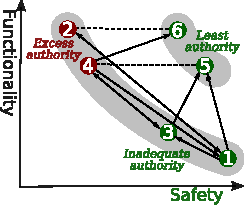
\includegraphics{seesaw-pola}}
  
\caption[The Evolving Authority of Active Content]{The Evolving Authority of 
Active Content. Identity-centric access controls have led to thrashing 
between lost functionality and lost safety. To have both, we need to provide 
\emph{least authority}: adequate authority for desired functionality without 
excess authority which invites abuse. \\ } \hrule
  \label{fig:evo-auth}
\end{figure}

When a document contains live interactive programs, we say it contains 
\emph{active content}. The computer industry has spent over a billion dollars 
in failed attempts to support active content. But the success of web 
apps---themselves a form of active content---demonstrates that this dream was 
worth pursuing. Unfortunately, web developers today face a maze of complex 
security mechanisms that have, so far, prevented web apps themselves from 
supporting active content. To navigate our way out of this maze, we must 
first see how we got here.

Today's desktop operating systems all use some form of identity-centric 
access control~\cite{karp:abac-soa}, in which an installed application runs 
\emph{as} its user, and so is entrusted with all its user's authority. Such 
an application can provide its user all the functionality modern operating 
systems support, but at the price of being able to do anything its user may 
do. We depict this situation at~\q{2} on Figure~\ref{fig:evo-auth}. When you 
run Solitaire, it can delete all your files while playing within the rules of 
your system, without exploiting any bugs. (For the remainder of this 
document, we will ignore hazards due to implementation bugs, and explain only 
hazards due to architectural choices.)

At first, the documents handled by applications were safe passive data~\q{1}. 
Applications first supported active content by running scripts in documents 
with all of their user's authority~\qq{1}{2}. Excess authority invites abuse. 
Simply ``reading'' a malicious document would allow it to delete all your 
files. In reaction, installed office applications now encourage users to 
disable scripts (Figure~\ref{fig:dialog}) reducing content back to passive 
data~\qq{2}{1}. The failures of excess authority shown on the upper left thus 
led to the failures of inadequate authority shown on the lower right.

The web browser is itself an installed application that runs scripts in two 
contexts. Browser extensions run with all the user's authority~\q{2}. Scripts 
in web pages run sandboxed, with no authority to the user's local files. The 
browser's \emph{same origin policy}, another layer of identity-centric 
control~\cite{mashupos}, provides scripts with the authority to communicate 
with their site of origin~\qq{1}{3}. Regarding both decisions, the user is 
helpless. The user has no practical way to grant a script the authority to 
edit one of the user's local files, nor can the user deny a script the 
ability to call home. So long as the user's valuable assets were local, this 
model successfully protected the user.

\begin{figure}[t!]
  \resizebox{\columnwidth}{!}{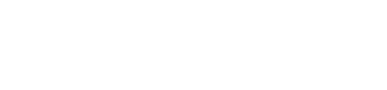
\includegraphics{dialog}}
  
\caption[Only Bad Choices.]{Only Bad Choices. When documents contain scripts, 
users can disable themselves from getting any work done \q{1} or enable 
scripts to destroy all their other work \q{2}. \\ } \hrule
  \label{fig:dialog}
\end{figure}

Web apps leverage this success. To the browser, the page on which a web app 
resides is a document, and the web app itself is simply active content within 
that document. But to the user, a web app is an application managing yet 
other documents on the user's behalf. For example, when the user interacts 
with webmail, the documents of interest are email messages. Likewise for 
groups, blogs, chat, docs and spreadsheets, wikis, and more. Let us refer to 
the documents managed by web apps as \emph{passages}, to distinguish them 
from the web pages on which they appear.

Since the user can neither grant a web app access to local files nor deny it 
the ability to call home, the only place a web app could store these passages 
is on its site of origin. The browser security model protected the user's 
local files from being harmed \emph{or used}. As users shift to using web 
apps, the assets they value come to be the passages stored at these various 
origin sites. 

To protect their user's remote passages, web apps employed yet another layer 
of identity-centric controls, relying on cookies or other forms of 
authentication to identify their user. But when scripts within these passages 
ran, they would run within the web page containing the web app serving them, 
and were thereby authorized to do anything their web app could do on behalf 
of its user~\q{4}. For example, if a webmail application allowed HTML email 
messages to carry scripts, simply ``reading'' an incoming email message would 
allow it to delete your inbox. The~\qq{3}{4} transition is not a technical 
change, but a change in where the user's value resides, and thus a change in 
the user's risks. By this dynamic, failures of inadequate authority led to 
failures of excess authority.

To protect against malicious passages, some web apps do safely provide active 
content using \emph{iframes}---effectively nested web pages---at the cost of 
isolating themselves from this content~\qq{4}{3}~\cite{mashupos}. Most web 
apps \emph{sanitize} HTML content by removing all scripts, reducing content 
again to passive data~\qq{4}{1}. Existing HTML sanitizers disinfect the 
patient but leave a corpse. This recapitulates the loss of active content in 
installed office applications. Some proposals would address these next 
incremental problems by adding yet another identity-centric 
epicycle. Can we do better?

\begin{figure}[t!]
  \resizebox{\columnwidth}{!}{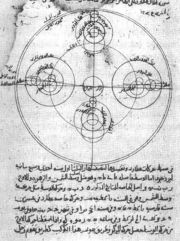
\includegraphics{epicycles}}

  \caption[Ptolemy's epicycles.]{Ptolemy's epicycles. Ptolemy attempted to
  model the motion of the heavenly bodies using only circles. With each
  discovery that the model didn't fit, yet another layer of circle was added
  to adjust. By contrast, Kepler's ellipses fit the problem directly, with no
  need for endless additional layers. 
  \\ } \hrule
  \label{fig:epicycle}
\end{figure}

If we could start over again, we could use an authorization-centric model 
such as object-capabilities~\cite{DVH}. The object-capability alternative 
naturally supports POLA, the principle of least authority, shown in the upper 
right of Figure~\ref{fig:evo-auth}. An object in an object-capability 
language can only cause effects by invoking the public interfaces of objects 
it can reach. An invocation provides references to other objects as 
arguments, providing the invoked object the least authority needed to carry 
out these requests~\cite{RobustComposition}. Within these rules, active 
content would run with exactly the authority explicitly provided by its 
containing document. Surprisingly, we can gain these benefits simply by 
applying a milder, non-lethal sanitizer.

Experience with Java, Scheme, OCaml, Pict, Perl and others demonstrates that 
existing memory safe languages often already contain an expressive 
object-capability subset~\cite[respectively]{joe-e, rees96security, emily, 
backwater, caperl}. We refer to the object-capability subset of JavaScript as 
\emph{Caja}. This subset is still a general purpose object programming 
language which JavaScript programmers should find familiar, pleasant, 
expressive, and easy to learn and use. 

Some web apps could use the Caja sanitizer to allow active content in their 
passages~\qq{1}{5}. Other web apps could use Caja to overcome the limits of 
iframes~\qq{3}{5}. Browser extensions, which run with their user's full 
authority, could make a \emph{powerbox} available to scripts in 
pages~\cite{darpareview, stiegler:polaris, seaborn:plash, bitfrost}. A web 
app, on detecting the presence of a powerbox, could offer to edit a local 
file chosen by the user~\qq{4}{6}.

\section{Subsetting JavaScript}
\label{sec:subset}

\begin{figure}[t!]
\begin{alltt}
function Counter()\ \{
  var count = 0;
  return caja.freeze(\{
    toString: function()\ \{ 
      return "<counter: " + count + ">"; 
    \},
    incr: function()\ \{ 
      return count += 1; 
    \},
    decr: function()\ \{ 
      return count -= 1; 
    \}
  \});
\}
\end{alltt}

\caption[A Cajita Counter.]{A Cajita Counter. Each call to \code{Counter()} 
produces a new counter object. Access to a counter provides the authority to 
read, invoke, or enumerate its properties, all of which are simple functions 
serving the role of methods. Caja functions are implicitly frozen; the 
returned object is explicitly frozen; and the instance-state of the 
object---the count variable---is accessible only as encapsulated state 
captured by these pseudo-methods. A counter object as a whole, as well as 
each of its pseudo-methods, are thus proper protected capabilities. Someone 
with access only to a counter's \code{incr} function can increment 
\emph{that} counter and observe the result, but not do anything else.
% XXX Confusing. Needs clarification
 \\ } \hrule
\label{fig:cajita-counter}
\end{figure}



Our starting point is JavaScript as documented in the third edition of the 
EcmaScript 262 standard~\cite{ECMA-262}; hereafter \emph{ES3}\footnote{
%
ES3 is approximately a bit more than JavaScript 1.4 and a bit less than 
JavaScript 1.5.
%
}.  ES3 code is passed to a Java program known as the the Caja sanitizer, 
or ``cajoler\footnote{
%
We thank Pat Patternson for this term.
%
}''.  The first set of restrictions is enforced by a static verifier. 
These restrictions mostly involve the use of trailing underscores, 
where the keyword ``\code{this}'' may appear, and the class definition pattern.
The second set of restrictions is imposed at runtime.  After statically 
verifying the code, the cajoler rewrites the code, inserting dynamic 
checks throughout. These involve restricting access to private members, 
forbidding modification of frozen objects, and so forth.  The actual 
logic of the runtime checks is contained in a runtime library, 
\code{caja.js}, that must be loaded by the JavaScript interpreter before 
loading a Caja module.

The remainder of this document explains the differences between Caja---the 
JavaScript subset accepted by the Caja sanitizer---and ES3. Other documents 
will explain the interface between cajoled and uncajoled JavaScript, and 
Caja's sanitization of the remaining elements of active web content: HTML, 
CSS, and the DOM and other APIs provided by browsers to JavaScript. We refer 
collectively to the subset of these accepted by the Caja sanitizer as 
\emph{Caja web content}, and to the sanitizer's corresponding output as 
\emph{Cajoled web content}.

\subsection{The OS analogy}
\label{subsec:os-analog}

A web app (or any other JavaScript-based embedding application framework) can 
be written partially in JavaScript and partially in Caja. The web app must load 
the Caja runtime library, which is written in JavaScript. All 
untrusted scripts must be provided as Caja source code, to be statically 
verified and cajoled by the Caja sanitizer. The sanitizer's output is 
either included directly in the containing web page or loaded by the Caja 
runtime.

A loose analogy with machine and operating system architecture may help 
explain the relationships. In the analogy, the full JavaScript language 
serves the role of the machine's full instruction set. JavaScript's global 
environment serves the role of physical memory addresses. The I/O-capable 
objects provided to JavaScript by a hosting environment, such as the DOM 
objects provided by the browser, serve the role of devices.

\begin{description}

  \item[User-mode.] By a combination of static and dynamic checks, the Caja 
  sanitizer allows only a safe ``user-mode'' subset of JavaScript. As with 
  user-mode instructions, this subset can compute any computable function, 
  but cannot cause external effects nor sense the outside world.

  \item[Address mapping.] A package of Caja source code to be cajoled 
  together defines a Caja module. All code within the same module 
  shares a global environment, but distinct modules see disjoint global 
  environments. The Caja sanitizer implements this by
  rewriting free variables as properties of a container-provided 
  ``imports'' object.

  \item[Context switching.] When Caja object A has a reference to Caja 
  object B, this should enable A to invoke B's public interface but not 
  access B's internal state. A and B should both be able to defend their 
  integrity from the other's possible misbehavior.

  \item[System calls, device drivers.] When a Caja object A invokes an 
  object B written directly in JavaScript, the operations provided by B serve 
  the role of system calls. Caja protects B from A, but A is fully 
  vulnerable to B. When B is a safe wrapper around one of the host's 
  device-like objects, such as a DOM node, B also serves as a device driver.

\end{description}

A ``system call'' corresponds to a Caja object invoking a JavaScript object. 
A web app that is written entirely in JavaScript and provides many services 
to its Caja objects directly would be like a monolithic kernel. For 
compatibility with existing JavaScript apps, we support this usage pattern 
but we don't recommend it. By analogy with kernel code at the boundary with 
untrusted code, such JavaScript code needs to maintain delicate invariants 
that it is easy to get wrong.

The other extreme is analogous to a micro-kernel. The minimal necessary 
JavaScript code would be the app-neutral Caja runtime itself, and a small 
app-dependent powerbox providing device drivers and initialization. All other 
services should be Caja objects to be invoked by other Caja objects. Most 
of the logic of a web app should be structured as such Caja-based services.

\subsection{JavaScript specific problems}
\label{subsec:js-probs}

Most of the above remarks would apply equally well were we starting from 
various other base languages. There are additional issues peculiar to 
JavaScript that we must deal with. Many of these issues are also software 
engineering hazards for which JavaScript programmers have developed 
defensive programming conventions. Where possible, Caja copes with these 
issues by adapting and enforcing these existing conventions.

\begin{figure}[t!]
\begin{alltt}
function Point(x, y)\ \{
  return caja.freeze(\{
    toString: function()\ \{ 
      return "<" + x + "," + y + ">"; 
    \},
    getX: function()\ \{ return x; \},
    getY: function()\ \{ return y; \},
  \});
\}

var ptA = Point(3, 5);
var ptB = Point(4, 7);
\end{alltt}

\caption[A Cajita Point.]{A Cajita Point. As a baseline, we first express 
this simple example in Cajita with no support for inheritance. Other 
elaborations will show how to support inheritance and various styles of 
definition in both Cajita and full Caja. 
\\ } \hrule
\label{fig:cajita-point}
\end{figure}

\begin{figure}[t!]
\begin{alltt}
function PointMixin(self, x, y)\ \{
  self.toString = function()\ \{ 
    return "<" + self.getX() + "," + 
                 self.getY() + ">"; 
  \};
  self.getX = function()\ \{ return x; \};
  self.getY = function()\ \{ return y; \};
  return self;
\}
function Point(x, y)\ \{
  return caja.freeze(PointMixin(\{\}, x, y));
\}
\end{alltt}

\caption[Cajita Inheritance.]{Cajita Inheritance. In the Cajita inheritance 
pattern, the equivalent of a non-final class is a function ending with 
``\code{Mixin}'' with \code{self} as its first parameter. The method-like 
functions can use \code{self} analogously to the use of \code{this} in full 
Caja, in order to refer to the overall object being defined. 
If the class is non-abstract, it should also have a pseudo-constructor function 
such as \code{Point} for making direct instances. This 
``\code{*Mixin}'' function should only be called by these pseudo-constructor 
functions, such as WobblyPoint in Figure~\ref{fig:cajita-super-wobbly-point}.\\ } \hrule
\label{fig:cajita-super-point}
\end{figure}

\begin{figure}[t!]
\begin{alltt}
function WobblyPointMixin(self)\ \{
  var super = caja.snapshot(self);
  self.getX = function()\ \{ 
    return Math.random() + super.getX(); 
  \};
  return self;
\}
function WobblyPoint(x, y)\ \{
  var self = PointMixin(\{\}, x, y));
  self = WobblyPointMixin(self);
  return caja.freeze(self);
\}
\end{alltt}

\caption[Cajita WobblyPointMixin.]{Cajita WobblyPointMixin. The equivalent of 
a non-final subclass is a ``\code{*Mixin}'' function with \code{self} as its 
first parameter, where the body calls \code{caja.snapshot} to make a frozen 
copy of the partially initialized \code{self} at that moment, to serve as the 
conventional \code{super} for the other functions defined within this scope. 
\\ } \hrule
\label{fig:cajita-super-wobbly-point} 
\end{figure}



\begin{description}

  \item[Unconstrained properties.] $\mbox{~~~~JavaScript objects}$ contain 
  \emph{properties}, i.e., named fields holding references to other objects. 
  JavaScript specifies that some properties are constrained to be 
  \emph{Protected}, \emph{ReadOnly}, \emph{DontEnum}, or \emph{DontDelete}. 
  Such constraints would help an object protect itself from its clients, but 
  JavaScript provides no way to express these constraints in the language. 
  Instead, any user-defined object in JavaScript is freely mutated by any other 
  object with access to it.
  
  \item[Global environment.] All JavaScript code executing within the same 
  JavaScript engine (such as a web page or iframe) implicitly share access to 
  the same global environment. Therefore, in JavaScript, objects cannot be 
  isolated from each other.

  \item[Implicit mutable state.] Some base JavaScript objects, such as 
  \code{Array.prototype}, are implicitly reachable even without naming any 
  global variable names. Even after global environment problems are fixed, 
  the mutability of these objects would prevent isolation.

  \item[Lack of encapsulation.] To support the ``context switching'' 
  criterion explained in section~\ref{subsec:os-analog}, objects need 
  to be able to encapsulate their private state. JavaScript does provide 
  one such mechanism: lexical variables captured by nested functions. 
  For example, in the following code, the variable \code{secret} cannot
  leak or be changed:
\begin{alltt}
function makePointFunction(secret)\ \{
  return function(value)\ \{ 
    return value === secret;
  \}
\}  
\end{alltt}
  However, using this as the sole 
  encapsulation mechanism for object patterns conflicts with existing 
  JavaScript programming practice.

  \item[``this'' what?] JavaScript's rules for binding ``\code{this}'' depend 
  on whether a function is invoked by \emph{construction}, by \emph{method 
  call}, by \emph{function call}, or by \emph{reflection}. If a function 
  written to be called in one way is instead called in another way, its 
  ``\code{this}'' might be rebound to a different object or even to the 
  global environment.

  \item[Foreign for/in loops.] Caja has a stated goal of supporting as much legacy code as possible, where it
  is safe to do so.  Nearly all Javascript libraries use JavaScript's \code{for}/\code{in} loop to enumerate the names of all an object's 
  properties, whether inherited or not\footnote{
  %
  ... unless the property is DontEnum, but the JavaScript programmer has no way to express that in his own code.
  %
  }. As a result, the properties used by the internals of the Caja runtime library, which are hidden to Caja code, 
  need to be skipped by the loop body. Every JavaScript coding style invents its own defensive pattern of additional 
  tests to skip unwanted property names.
  
  Though not part of Caja itself, the Caja distribution includes an ``innocent code'' transformer that parses JavaScript and
  surrounds the body of all \code{for/in} loops with a check that skips properties internal to the Caja library---\emph{i.e.}
  properties ending in ``\_\_\_'', triple underscore.
    
  \item[Weak static analysis.] Although Caja is less dynamic than JavaScript, we still assume that it is impractical 
  to perform any interesting analysis, such as type inference, both statically and safely. As a result, Caja's static 
  restrictions can only enforce simple syntactic rules. Remaining restrictions must be enforced by runtime checks.
  
  \item[Fast path.] For the micro-kernel approach to be attractive, Caja's extra runtime checks must not cost too 
  much. Frequent operations, such as property access using ``.'' must run close to full speed.
  
  \item[Uncontrolled language growth.] The ES3 spec allows one to add new dangerous properties to core objects while 
  claiming ES3 compatibility. JavaScript language implementors, platform providers, and standards committees make use 
  of this freedom with unpredictable results. For example, some JavaScript implementations have added dangerous 
  properties, like \code{eval}, to core objects, like \code{Object.prototype}. A safe subset must deny access to 
  these additional unknown properties. But since these new properties are often DontEnum, there isn't even a reliable 
  way to detect them.
  
  \item[Browser compatibility.] Web content must work on widely deployed browsers whether on not these browsers 
  strictly conform to the relevant standards. At the time of this writing, the plausible baseline platform is 
  Yahoo!'s list of A-Grade browsers /cite{Yahoo:AGrade}. Fortunately, these browsers do conform closely to ES3. 
  Later versions of Caja may specify larger subsets of ES3.
  
  \item[Multiple worlds.] As with many languages, each instantiation of a JavaScript language world creates a set of 
  primordial objects (like \code{Object.prototype}) that are global to that world. Unlike other languages, JavaScript 
  is built to support multiple interacting worlds. For example, in the browser environment, a new JavaScript world is 
  created for each iframe. An object from one iframe can hold a direct reference to an object from another iframe of 
  the same origin. This leads to some surprises. Even if \code{x} holds an array, \code{x instanceof Array} may 
  evaluate to false because \code{x} is an instance of the \code{Array} from a different JavaScript world.
  
  \item[Silent errors.] In JavaScript, various operations, such as setting a ReadOnly property, fail silently rather 
  than throwing an error. Program logic then proceeds along normal control flow paths premised on the assumption that 
  these operations succeeded, leading to inconsistency. To program defensively in the face of this hazard, every 
  assignment would be followed by a ``\emph{did it really happen?}'' test. This would render programs unreadable and 
  unmaintainable. Where practical, Caja deviates from standard JavaScript by throwing an exception rather than 
  failing silently.
  
  \item[Object detection.] In JavaScript, reading a non-existent property returns \code{undefined} rather than 
  throwing an exception. The JavaScript \emph{object detection}\footnote{
  %
  See {\tt http://www.quirksmode.org/js/support.html}.
  %
  } pattern relies on this behavior. Since, in this case, 
  the program naturally notices the problem anyway, Caja does not turn this case into a thrown exception.
    
\end{description}

The above point about ``Silent errors'' is another reason to avoid the monolithic kernel approach. Web apps in 
uncajoled JavaScript are vulnerable to any malicious active content that finds a way to provoke a silent error and 
exploit the resulting inconsistency.

\subsection{A fail-stop subset}
\label{subsec:fail-stop}

There are four ways that the semantics of cajoled code may differ from those of uncajoled code.
First, it may fail to pass the static verifier; second, it may throw an exception at runtime; third, it
may return \code{undefined} when trying to read a protected variable from outside the encapsulating
object; and fourth, by hitting one of a few rare corner cases where the semantics have to differ in order
to preserve the security properties.  We call the last set of deviations ``gotchas'', and detail them
in sections \ref{subsec:cajita-gotcha} and \ref{subsec:caja-gotchas}.  Since (in all cases but the gotchas) 
the semantics differ only when there is an error, or ``failure'', Caja is a \emph{fail-stop subset}\footnote{
%
We thank Dan Rabin for this formulation.
%
} of ES3.

A \emph{Caja-compliant} JavaScript program is one which
\begin{enumerate}
  \item is statically accepted by the Caja sanitizer,
  \item does not provoke Caja-induced failures when run cajoled, and
  \item avoids these gotchas.
\end{enumerate}
Such a program should has the same semantics whether run cajoled or not.


\section{Cajita Specification}
\label{sec:cajita-spec}
Before describing Caja and all the Rube-Goldbergian complexity of the
semantics of ``\code{this}'', we'll describe the subset of Caja without 
``\code{this}''---a perfectly reasonable and expressive programming 
language. Caja supports ``\code{this}'' in order to ease the porting of old 
code. For new code, we recommend sticking to Cajita\footnote{
%
The design of Cajita was inspired by Doug Crockford's \emph{ADsafe}.
%
}.

The Caja runtime will provide a safe \emph{eval} operation, \code{caja.cajitaEval}. For 
this operation to accept Caja code, the Caja sanitizer would need to be 
written in JavaScript and included in the Caja download. To minimize download 
size, \code{caja.cajitaEval} will instead accept only Cajita code.

To explain the restrictions Cajita imposes, we need some definitions.

\begin{description}

  \item[Record.] An object whose prototype's ``\code{constructor}'' property is \code{Object}, i.e., under normal 
  conditions, an object inheriting directly from \code{Object.prototype}. Records are normally created using the 
  \code{\{\ldots\}} syntax.

  \item[Array.] An object whose prototype's ``\code{constructor}'' property is \code{Array}, i.e., under normal 
  conditions, an object inheriting directly from \code{Array.prototype}. Arrays are normally created using the 
  \code{[\ldots]} syntax.

  \item[JSON Container.] A record or array. These are the non-primitive objects that can be directly expressed in 
  JSON syntax.  Note: whenever the word ``container'' appears unqualified, we are referring to the \emph{module
  container}, not a JSON container.
  
  \item[Function.prototype.bind.] Cajita and Caja add the \code{bind} method to all functions, defined in equation
  \ref{eq:sf-bind-n} of figure \ref{eqn:simple-func}.  The popular Prototype library, ES3.1, and ES4 all define \code{bind}
  in this way.
  
  \item[Invocation.] A function can be invoked
  \begin{itemize}
    \item \emph{as a function} (\code{foo(a\ldots)}),
    \item \emph{as a method} (\code{foo.m(a\ldots)}),
    \item \emph{as a constructor} (\code{new Foo(a\ldots)}), or
    \item \emph{reflectively} (by calling its \code{call}, \code{apply}, or \code{bind} methods).
  \end{itemize}

  \item[Simple functions.] A function whose body does not mention ``\code{this}'' is a \emph{simple function}. A 
  simple function can be either named or anonymous. Simple functions are first-class---they can be stored in 
  variables and passed around freely, just like any other value.
  
  \item[Frozen.] If an object is \emph{frozen}, any attempt to directly assign to its properties, add new properties 
  to it, or delete its properties causes an exception to be thrown. Frozen is a shallow restriction: Frozen objects 
  can retain and provide non-frozen objects. (Imagine a frozen surface covering a liquid lake.) In Cajita and Caja, functions  
  are implicitly frozen once they've been intitialized. The Caja runtime library additionally provides an explicit 
  operation for freezing JSON containers: ``\code{caja.freeze(obj)}''.
  
  \item[Immutable.] If an object is \emph{immutable}, then it is frozen, and all objects it has access to are 
  themselves immutable. Shared access to an immutable object does not provide a communication channel, and so does 
  not endanger isolation. With the exception of \code{Math.random} and \code{Date}, all objects that are globally or 
  implicitly accessible to all Caja programs are immutable. We discuss these exceptions in 
  section~\ref{subsec:outer-env}.

\end{description}

\subsection{Cajita regularities}
\label{subsec:cajita-reg}

\begin{figure}
\begin{eqnarray}
  \code{F(\ldots)}                & \equiv & \code{new\ F(\ldots)}                     \label{eq:sf-new} \\
                                  & \equiv & \code{F.call(v,\ldots)}                   \label{eq:sf-call} \\
                                  & \equiv & \code{F.apply(v,[\ldots])}                \label{eq:sf-apply} \\
                                  & \equiv & \code{F.bind(v)(\ldots)}                  \label{eq:sf-bind-1} \\
  \code{F({\ldots}_1,{\ldots}_2)} & \equiv & \code{F.bind(v,{\ldots}_1)({\ldots}_2)}   \label{eq:sf-bind-n} \\
  \code{x.m}                      & \equiv & \code{true\ \&\&\ x.m}                    \label{eq:sf-true} \\
  \code{(x.m)(\ldots)}            & \equiv & \code{(true\ \&\&\ x.m)(\ldots)}          \label{eq:sf-true-call} \\
  \code{\{\ldots\}}               & \equiv & \code{(function()\{{\ldots\}})()}         \label{eq:sf-thunk-stmt} \\
  \code{(\ldots)}                 & \equiv & \code{(function()\{return\ {\ldots\}})()} \label{eq:sf-thunk-expr}
\end{eqnarray}

\caption[Cajita Regularities.]{Cajita Regularities. Given that \code{F} is a simple function, \code{x.m} holds a 
simple function, and \code{v} is an expression with no effects and stable value (such as a variable reference), then 
most of these equivalences hold in Caja as well as Cajita. Equation~(\ref{eq:sf-thunk-stmt}) 
holds in general only in Cajita. See section~\ref{subsec:cajita-reg} for further qualifying conditions. \\ } \hrule
\label{eqn:simple-func}
\end{figure}

The regularities in Figure~\ref{eqn:simple-func} apply when calling simple functions, whether the 
calling code is in Cajita or Caja. When calling other functions, only the 
weaker \emph{Caja regularities} shown in Figure~\ref{eqn:caja-regularities} apply. The 
regularities in both sections are often stronger than ES3, but are all within 
a fail-stop subset of ES3.

\begin{itemize}
  \item Equation~(\ref{eq:sf-new}) of Figure~\ref{eqn:simple-func} states that the \code{new} keyword does not change 
  the meaning of calling a simple function. This holds only for simple functions that explicitly \code{return} a 
  value. As in uncajoled JavaScript, if a simple function instead implicitly returns, it will return \code{undefined}
  when called without \code{new}, but will return a useless object when called with \code{new}.
  
  \item Equation (\ref{eq:sf-thunk-expr}) holds in Cajita and Caja when the left-hand side does not mention \code{arguments} freely.
  
  \item Equation (\ref{eq:sf-thunk-stmt}) holds only in Cajita, and only when the left hand side does not contain 
  a free break, a free continue, or a return statement.
    
  \item When calling the \code{call}, \code{apply}, or \code{bind} method of a simple function, the first argument is 
  ignored: a simple function cannot contain the keyword \code{this} and thus has no way to refer to that argument.
  
  \item The \code{apply} method differs from \code{call} only in packaging all arguments together into a list.
  
  \item A single-argument \code{bind} of a simple function returns a function with equivalent invocation behavior---a 
  function that behaves the same, whether called as a function, as a constructor, as a method, or reflectively.
  
  \item When \code{bind} has additional arguments, it returns a new function representing \code{F} curried over these 
  additional arguments.
  
  \item In JavaScript, when the left operand of an \code{\&\&} expression evaluates to a ``truthy'' value---that is,
  any value \code{x} such that \code{Boolean(x) === true}---the \code{\&\&} 
  expression as a whole evaluates to the value of its right operand. Therefore, you might expect 
  Equation~(\ref{eq:sf-true}) to hold in general. The next item sheds light on why it does not hold in JavaScript 
  when the value of the right operand is a non-simple function.

  \item In JavaScript, when the value of a property \code{x.m} is a function, the expression \code{(x.m)(...)} 
  binds \code{this} to \code{x}, whereas \code{(true \&\& x.m)(...)} binds \code{this} to the global scope. 
  In a web browser, the global scope is reified as the object \code{window}, so the browser calls \code{m} 
  as a method on \code{window} instead of on \code{x}.  Fortunately, when \code{m} is a simple function, 
  these two forms of invocation have the same meaning.

\end{itemize}



\begin{figure}[t!]
\begin{alltt}
function Brand()\ \{
  var flag = false, payload = null;

  return caja.freeze(\{
    seal: function(payloadToSeal)\ \{
      function box()\ \{
        flag = true; 
        payload = payloadToSeal;
      \}
      box.toString = function()\ \{
        return "(box)";
      \};
      return box;
    \},
    unseal: function(box)\ \{
      flag = false; 
      payload = null;
      try \{
        box();
        if (!flag) \{ throw {\ldots}; \}
        return payload;
      \} finally \{
        flag = false; 
        payload = null;
      \}
    \}
  \});
\}
\end{alltt}

\caption[Rights Amplification]{Rights Amplification. Each brand has a 
\code{seal} and \code{unseal} function, acting like a matched encryption and 
decryption key. Sealing an object returns a sealed \code{box} that can only 
be unsealed by the corresponding \code{unseal} function. The implementation 
technique shown here is due to Marc Stiegler.
\\ } \hrule
\label{fig:rights-amp}
\end{figure}



\subsection{Common static restrictions}
\label{subsec:common-static}

Any source code statically accepted by the Caja sanitizer is a \emph{legal 
Caja program}. A legal Caja program satisfying additional static restrictions 
is also a \emph{legal Cajita program} and will be accepted by the Cajita 
sanitizer. A Caja-compliant JavaScript program that is also a legal Cajita 
program is a \emph{Cajita-compliant JavaScript program}---it will have the 
same semantics whether uncajoled, cajoled by the Caja sanitizer, or cajoled 
by the Cajita sanitizer.

The static restrictions immediately below apply to both Caja and Cajita. This 
is followed by the additional static restrictions specific to Cajita.

\begin{description}

    \item[Stable language.] Virtually any input which should be statically 
    rejected by ES3 is forbidden, even if it would be allowed by a target 
    browser or later JavaScript specifications. This includes any use of 
    keywords reserved in ES3. But we reserve the right to include 
    \emph{de-facto extensions} to ES3 as explained below.
    
    \item[De-facto extensions.] As we identify widely supported extensions of 
    ES3 that we can accept as input, but still cajole to conforming ES3 on 
    output, we may add these to Caja. For example, we are currently 
    considering allowing backslash as a line continuation character, since 
    this is allowed by virtually all JavaScript implementations and can be 
    trivially cajoled to correct ES3.

    \item[Without ``with''.] The ``\code{with}'' keyword is forbidden. 
    Because of the scope confusion it causes, ``\code{with}'' is a widely 
    hated and avoided feature that would be a lot of trouble to support 
    safely.

    \item[Beware unicode.] Cajita and Caja accept unicode characters only in 
    string literals.  Some of these create parsing 
    problems on some widely deployed JavaScript platforms. Prohibiting these 
    protects against some character-encoding attacks. We expect to relax this 
    restriction once we know how to do so safely.

    \item[Forbidden names.] An identifier ending with a double underscore is 
    forbidden, either as a variable name or a property name. We reserve the 
    triple underscore for use by the sanitizer's cajoled output and by the 
    Caja runtime. Firefox reserves the double underscore for itself.
    
    \item[``new'' is ok.] Since Cajita does not have \code{this}, 
    constructors, nor prototypes, \code{new} isn't needed purely within 
    Cajita. But since Cajita code must interoperate smoothly with Caja and 
    uncajoled JavaScript code, \code{new} is considered a valid part of 
    Cajita.
    
    \item[No assignment to imports or declared functions.]  Variables used freely
    in Caja code refer to properties of the \code{IMPORTS\_\_\_} object, and
    assignment to these properties is statically rejected.  Declared function names
    may not be reassigned.  For example, the following code is illegal in Cajita
    and Caja:
\begin{alltt}
function foo() {}
foo = 3;
\end{alltt}
    
  \item[No deleting variables.]  Allowing variables to be deleted prevents
  static scope analysis, so Cajita and Caja both prohibit it.  Properties 
  of objects, however, may still be deleted.
        
\end{description}

\begin{figure}[t!]
\begin{alltt}
function Mint()\ \{
  var brand = Brand();
  return function Purse(balance)\ \{
    caja.enforceNat(balance);
    function decr(amount)\ \{
      caja.enforceNat(amount);
      balance = 
        caja.enforceNat(balance-amount);
    \}
    return caja.freeze(\{
      getBalance: function()\ \{
        return balance; \},
      makePurse: function()\ \{
        return Purse(0); \},
      getDecr: function()\ \{
        return brand.seal(decr); \},
      deposit: function(amount,src)\ \{
        var box = src.getDecr();
        var decr = brand.unseal(box);
        var newBal = 
          caja.enforceNat(balance+amount);
        decr(amount);
        balance = newBal;
      \}
    \});
  \}
\}
\end{alltt}

\caption[The MintMaker Example]{The MintMaker Example. Calling \code{Mint()} 
creates a \code{Purse} function for making purses holding new transferable 
units of a distinct ``currency''. Given two purses of the same currency, one 
can transfer money between them, but one can't violate conservation of 
currency. \\ } \hrule
\label{fig:mintmaker}
\end{figure}

% XXX fig:rights-amp and fig:mintmaker need more explanation

\subsection{Cajita-only static restrictions}
\label{subsec:cajita-only-static}



The following features are present in Caja in order to accommodate old code, 
rather than to enhance expressiveness. Since Cajita is for new code, in order 
to minimize the dowload size of the Cajita sanitizer, as well as to simplify 
the semantics of Cajita considered on its own, these features are absent from 
Cajita. Code containing these features is not legal Cajita.

\begin{description}
    
    \item[``this''.] The central difference between Caja and Cajita is that only Caja includes ``\code{this}''.
    
    \item[Protected names.] In Caja, an \emph{protected name} is a property name ending in ``\code{\_}'' (a single 
    underbar). Such names are used for encapsulation in Caja but are prohibited in Cajita. Cajita's only 
    encapsulation mechanism is lexical scoping.
    
    \item[Prototypes.] In Caja and Cajita, if ``\code{Foo}'' is a function name, then static properties of the 
    function can be initialized until the first time the function is used. Cajita prohibits access to \code{Foo}'s 
    ``\code{prototype}'' property, and so prevents use of JavaScript's prototype inheritance within Cajita.
    
    \item[``instanceof''.] Without ``\code{this}'' and prototypes, Cajita has no need for \code{instanceof}. Rather, 
    JavaScript's \code{typeof} is almost an adequate type discriminator for Cajita. But Cajita still needs a way to 
    distinguish records from arrays. We could allow the conventional \code{x instanceof Array} expression, but it 
    does not work correctly when \code{x} is an array from another cajoled JavaScript world, such as another iframe 
    with the same origin. Instead we provide \code{caja.isArray(x)} as a correct alternative.
    
    \item[Literal RegExp syntax.] In JavaScript implementations, the literal pattern syntax is often optimized into a 
    static object with mutable state, violating isolation. The Caja sanitizer cajoles the \code{/pattern/} syntax to 
    \code{new RegExp("pattern")}. In Cajita, the second form must be written explicitly.
    
    \item[for/in loops.] Because of the confusing semantics of JavaScript's \code{for/in} loops, these are absent 
    from Cajita. Instead, Cajita code should enumerate the properties of \code{obj} by doing
%
\begin{alltt}caja.forEach(obj,function(v,k)\{{\ldots}\});\end{alltt}
%
    This code will reliably give the same results whether run cajoled or not. It will enumerate only the 
    non-inherited publicly Caja-visible property value / property name associations of \code{obj}. If 
    \code{caja.isArray(obj)}, then \code{k} will enumerate successive indexes into the array.
    
    \item[Semicolon insertion.] JavaScript will insert semicolons automatically in certain situations involving
    newlines. Code which parses correctly but differently if semicolons are automatically inserted is not legal Cajita.  
    For example, due to the newline at the end of the first line, this code
\begin{alltt}
x = a 
      + b;
\end{alltt}
    has two different correct parses: \code{x = a + b;} and \code{x = a; +b;}.  
    
    Therefore, code which has a newline between \code{x = a} and \code{+ b} is not legal Cajita.  
    It should be replaced by \code{x = a + b;} which is unambiguous.
    
    \item[Block-breaking scopes.] Cajita variable names are visible only according to the intersection of ES3's 
    scoping rules and conventional Java-like block-level lexical scoping. This is essentially lexical scoping from 
    the point of introduction with the restriction that a function cannot contain two definitions of the same 
    variable name, even in two separate blocks. If JavaScript scope analysis and conventional block-level lexical 
    scope analysis would disagree on the variable bindings of a given piece of code, then that code is not legal 
    Cajita.
    
    \item[Coercing equality.] JavaScript's coercing rules for the ``\code{==}'' and ``\code{!=}'' operators are 
    complex, accident prone, and not even transitive. Cajita only includes the equality operators ``\code{===}'' and 
    ``\code{!==}''.
        
\end{description}


\subsection{Cajita dynamic restrictions}
\label{subsec:cajita:dynamic}

The following restrictions apply to both Caja and Cajita.

\begin{description}

  \item[Frozen Functions.] An anonymous simple function is implicitly frozen. 
  A named simple function may be initialized, but is implicitly frozen 
  immediately before its first non-initializing use or escaping occurrence. 
  For example, the assignment to \code{box.toString} in 
  Figure~\ref{fig:rights-amp} will succeed, because it occurs before box is 
  implicitly frozen by the following \code{return} statement. Initializing 
  assignments can thus be considered declarative initializations rather than 
  mutations.
  
  \emph{Claim: No Caja program can cause a Caja-observable mutation of a 
  function or of any object Caja considers frozen.}
  
\end{description}


\subsection{Modules}
\label{subsec:outer-env}

The output of the Caja sanitizer consists almost entirely of a JavaScript function 
called a \emph{module}.  The \emph{bound} variables of a module are those that appear as the names of
functions declared in the Caja code or in a \code{var} declaration.  The \emph{free}
variables are the variables that are not bound.  

One of the arguments of every module function is named \code{IMPORTS\_\_\_}, and the 
Caja sanitizer rewrites all free variables to be properties of \code{IMPORTS\_\_\_}.  
For example, the cajoling process rewrites
\begin{alltt}
var list = new Foo(6);
\end{alltt}
to (approximately)
\begin{alltt}
var Foo = ___readPub(IMPORTS\_\_\_, 'Foo');
var list = new (___.asCtor(Foo))(6);
\end{alltt}
From the container's perspective, this effectively reifies the module's global scope.
Note that the module itself does not necessarily have a means of obtaining a reference 
to \code{IMPORTS\_\_\_}.

If a container wants to allow communication between two modules, it can provide
a mutable object as a property of \code{IMPORTS\_\_\_}, say, 
\begin{alltt}
IMPORTS\_\_\_.channel = \{\};
\end{alltt}
Then if one module sets a property of \code{channel} in its code, the other can read
the property and vice-versa:
\begin{alltt}
// In module 1:
channel.message = "Hi there!";

// In module 2:
alert(channel.message);
// Displays "Hi there"
\end{alltt}

Similarly, if the container wishes to grant a module reified access to its \code{IMPORTS\_\_\_},
it can set, for example, \code{IMPORTS\_\_\_.global = IMPORTS\_\_\_}.

\emph{Claim: Two separate module instances, even if they instantiate the same module, 
are isolated from each other unless they have been granted references to the same mutable object.}

Here are some restrictions that the \code{IMPORTS\_\_\_} object must have in order
to preserve Caja's security properties.
\begin{description}

    \item[eval]  The whole point of the cajoler and runtime library is to enforce
    the Caja restrictions on JavaScript.  The \code{eval} method would allow
    arbitrary JavaScript to be executed, so it's important that a Caja module never
    gets a reference to the \code{eval} method.
    
    Instead, ``\code{caja.cajitaEval}'' will evaluate Cajita source code (text or 
    AST).  The \code{cajitaEval} function will take an \code{imports} object, and
    free variables in the source will be bound to properties of \code{imports}.
    
    \item[Function] The JavaScript \code{Function} constructor is absent 
    for the same reason as \code{eval}.
    
    \item[Restricted reflection] Allowing access to the \code{constructor} property of 
    prototypical objects and functions would grant the authority to create more objects like them,
    which violates the principle of least authority.  Therefore, the built-in \code{constructor} 
    property is absent from Caja. 
    
    The \code{prototype} property of functions can only be
    used in the limited\footnote{
    %
    See \myurl{http://code.google.com/p/google-caja/issues/} \\
    \myurl{detail?id=346} for details of the attack enabled by unrestricted access.
    %
    } ways shown in Figure~\ref{tab:special-cases}. 
    
    The \code{call}, \code{apply}, and
    \code{bind} methods of functions cannot be replaced or overridden.
    
    \emph{Claim: The restrictions stated in this document together make the 
    \code{Function} object unreachable from Caja programs.}

    \item[new Date()] Nearly all of the members of the global environment
    are immutable.  However, in JavaScript, ``\code{new Date()}''  gives ambient 
    access to the current date and time, in violation of object-capability 
    rules as well as dependency injection discipline. \code{Date} is 
    therefore a member of the global environment which is not actually 
    immutable. Further, this ambient access to the current time provides a 
    timing channel, further impeding any attempts to stem the leakage of bits 
    over covert channels. Nevertheless, despite these concerns, because it 
    provides only a read-only channel for sensing the world, Caja provides 
    the JavaScript \code{Date} constructor to Caja programs.

    \item[Math.random()] The JavaScript \code{Math.random} method is not even 
    read-only. The ES3 standard places no obligations regarding quality of the
    randomness produced. In particular, an implementation could conform to ES3
    and still leak to a given caller of \code{Math.random()} the ability to
    infer how many previous times it had been called. Nevertheless, Caja
    provides the JavaScript \code{Math.random} method to Caja programs. We
    recommend that JavaScript platform providers provide good enough
    randomness that this method doesn't serve as an information channel
    between otherwise-isolated modules.
    
\end{description}


\subsection{Cajita gotchas}
\label{subsec:cajita-gotcha}

Caja seeks to define a fail-stop subset of ES3, as explained in section~\ref{subsec:fail-stop}. However, 
it falls short of this goal in several minor ways. To write a correct program 
that executes correctly whether run cajoled or uncajoled, it should 
avoid these gotchas. In this section, we enumerate those gotchas relevant to 
the Cajita subset of Caja.

\begin{description}

  \item[Snapshot ``arguments''.] In ES3, if \code{x} is the i'th parameter of 
  a function, assignments to \code{x} are visible as changes to 
  \code{arguments[i]} and vice versa. In Caja, if ``\code{arguments}'' is mentioned, it is 
  bound to a proper array snapshot of the arguments list when the function 
  was entered, \emph{not} an array-like object. In order for Caja to be a 
  fail-stop subset of ES3, a future version of the Caja sanitizer will 
  statically disallow assignments to any parameter variable within a function 
  that mentions ``\code{arguments}''. But in the initial Caja implementation, 
  this minor gotcha remains.
  
  \item[Absent ReferenceError.] In ES3, when a reference to an undefined 
  variable is evaluated as an expression, a \code{ReferenceError} is thrown. 
  The Caja sanitizer cajoles a reference to an undefined variable into a 
  reference to a property of \code{IMPORTS\_\_\_}. Given the current cajoling rules, a 
  reference to an undefined outer variable will evaluate to \code{undefined} 
  rather than throwing a \code{ReferenceError}. 
  
  \item[Top-level variable declaration is not an import.]  In JavaScript,
  free variables and declared variables at the top-level are both properties
  of the global object.  In Caja, even though free variables are rewritten 
  to properties of imports, declaring a variable with \code{var} does not 
  add a property to the \code{IMPORTS\_\_\_} object.

\end{description}

\section{Caja Specification}
\label{sec:caja-spec}

Whereas Cajita is a small subset of JavaScript meant to support new code, 
Caja is a large subset of JavaScript meant to ease the porting of old 
JavaScript code and practices. Cajita is small enough that its security 
properties can be understood. Caja seeks to accept as large a subset of 
JavaScript as is practical without losing the security properties provided by 
Cajita. In this section, we explain only the remaining elements of Caja 
beyond the elements of Cajita already explained.

To explain the remaining elements of Caja, we need some additional 
definitions.

\begin{description}

  \item[Constructed object.] An object defined by Caja code that's not a JSON 
  container and not a function must have been constructed by calling 
  ``\code{new}'' on a function other than \code{Array} or \code{Object}.

  \item[Prototypical objects.] As in ES3, a constructed object's implicit \emph{prototype}---the object it directly 
  inherits from---is the value of the \code{prototype} property of the function which constructed it (which must 
  have been called with ``\code{new}''). In Caja, these \emph{prototypical objects} are not first-class. When a 
  function is implicitly frozen, so is its \code{prototype}. Until then, both it and its \code{prototype} may be 
  initialized.

  \item[Constructors.] A named function whose body mentions ``\code{this}'' 
  is a \emph{constructor}. 
    
  \item[Methods.] An anonymous function whose body mentions ``\code{this}'' 
  is a \emph{method}.  A method definition may appear in one of two constructions.
  The first is as a parameter in the member map in a call to \code{caja.def}.
  For example, \code{getX} and \code{setX} are methods in the following code:
\begin{alltt}
function Foo(x)\ \{ this.x_ = x; \}
caja.def(Foo, Object, \{
  getX:function\ ()\ \{ return this.x_; \},
  setX:function\ ()\ \{ this.x_ = x; \}
\});
\end{alltt}
  
  The second is as the right-hand side of an assignment to a property of a
  constructor's prototype, before the constructor's first use.  For example:
\begin{alltt}
function Foo(x)\ \{ this.x_ = x; \}

// These are allowed
Foo.prototype.getX = function\ ()\{ 
  return this.x_; 
\};
Foo.prototype.setX = function\ (x)\{ 
  this.x_ = x; 
\};

// First reference to Foo
var f = new Foo(0);

// This is no longer allowed
Foo.prototype.add3 = function\ (x)\{
  return x + 2;
\};
\end{alltt}

  In both these cases, the function is marked as a method and is added as a
  property of object bound to the constructor's \code{prototype} property. Such
  a function is called an \emph{unattached method}, in contrast to an
  \emph{attached method}, explained below. Direct references to unattached
  methods should never be accessible to Caja code.
  
  When a method like \code{getX} is read as a property of an object \code{o}, it
  returns instead an \emph{attached method}, a wrapper around the unattached
  method that stores \code{o}; when it is invoked as a method on some object
  \code{o2}, the wrapper first verifies that \code{o === o2}.  If the two are
  not equal, then the wrapper throws an exception.
  
  An \emph{inline method} is an anonymous function mentioning ``\code{this}''
  that is immediately invoked using \code{call}, \code{apply}, or \code{bind}
  with ``\code{this}'' as the first parameter.  Inline methods are a means of
  achieving true block scoping in Caja. See section \ref{subsec:caja-reg} for
  more details.
\end{description}


\subsection{Caja regularities}
\label{subsec:caja-reg}

The regularities shown in Figure~\ref{eqn:caja-regularities} apply when Caja code calls any Caja function 
\emph{other than} a constructor. These regularities are often stronger than ES3, but are all within a 
fail-stop subset of ES3. 

\begin{figure}
\begin{eqnarray}
  \code{x.m(\ldots)}         & \equiv & \code{(true \&\& x.m).call(x,\ldots)}         \label{eq:caja-true-call} \\
                             & \equiv & \code{x.m.call(x,\ldots)}                     \label{eq:caja-call} \\
                             & \equiv & \code{x.m.apply(x,[\ldots])}                  \label{eq:caja-apply} \\
                             & \equiv & \code{x.m.bind(x)(\ldots)}                    \label{eq:caja-bind-1} \\
  \code{x.m.bind(x)}         & \equiv & \code{(true\ \&\&\ x.m).bind(x)}              \label{eq:caja-true-bind} \\ 
  \code{x.m({\ldots}_1,{\ldots}_2)} 
                             & \equiv & \code{x.m.bind(x,{\ldots}_1)({\ldots}_2)}     \label{eq:caja-bind-n} \\
  \code{(\ldots)}            & \equiv & \code{(function()\{}                          \label{eq:caja-thunk-expr} \\
                             &        & \code{\ \ return\ {\ldots\}}).call(this)}     \nonumber\\
  \code{\{{\ldots}\}}        & \equiv & \code{(function()\{}                          \label{eq:caja-thunk-stmt} \\
                             &        & \code{\ \ \ldots\}).call(this)}               \nonumber
\end{eqnarray}

\caption[Caja Regularities.]{Caja Regularities. In Caja, given that \code{x.m} is associated with either a 
simple function or a method, then these equivalences hold. See section~\ref{subsec:caja-reg} for qualifying conditions. \\ } \hrule
\label{eqn:caja-regularities}
\end{figure}

\begin{itemize}

  \item The code on the left of Equation~(\ref{eq:caja-true-call}) of Figure~\ref{eqn:caja-regularities} calls
  \code{x.m} as a method on \code{x}. The code on the right first extracts the value of \code{x.m}. When \code{x.m} 
  is a method, the extracted value is an \emph{attached method} whose attachment is \code{x}. When \code{x} is an 
  expression with no effects and a stable value (such as a variable reference), the code on the right then calls the 
  attached method's \code{call} method with its attachment and the original arguments. These two calls are equivalent.
  
  \item The \code{apply} method differs from \code{call} only in packaging all arguments together into a list.
  
  \item Binding an attached method to its attachment yields a conventional bound method---a simple function of the 
  remaining arguments which calls the original method as a method on its attachment.
  
  \item When \code{bind} has additional arguments, it returns a new function representing \code{F} curried over these 
  additional arguments.
  
  \item Equation (\ref{eq:caja-thunk-expr}) holds when the expression does not mention \code{arguments}.

  \item Equation (\ref{eq:caja-thunk-stmt}) holds when no \code{break}, \code{continue}, or \code{return} appears
  freely in the body and no variable defined in the body has the same name as a variable in scope outside the body.

\end{itemize}


\begin{figure}[t!]
\begin{alltt}
function Point(x, y)\ \{
  this.x\_ = x;
  this.y\_ = y;
\}
Point.prototype.toString = function()\ \{ 
  return "<" + this.getX() + "," + 
               this.getY() + ">"; 
\};
Point.prototype.getX = function()\ \{ 
  return this.x\_; 
\};
Point.prototype.getY = function()\ \{ 
  return this.y\_;
\};

var ptC = new Point(3, 5);
var ptD = new Point(4, 7);
\end{alltt}

\caption[A Caja Point.]{A Caja Point. The point example, written in this common class-like pattern of Javascript 
programming, is valid Caja. \code{Point} is frozen by its first use, after which neither \code{Point} nor 
\code{Point.prototype} can be further initialized. \\ } \hrule
\label{fig:caja-point}
\end{figure}


\subsection{Caja static restrictions}
\label{subsec:caja-static}

Any source code statically accepted by the Caja sanitizer is a \emph{legal 
Caja program}. The following syntactic explains why a program may instead be statically rejected.

\begin{description}

  \item[Protected properties.] A property name ending in a single underscore may 
  be used only to name protected properties. It may appear as a property name of 
  ``\code{this}''.
  
  \item[Constructor names.] A Caja constructor can only be called as a 
  constructor using \code{new}, in order to instantiate a direct instance, 
  or reflectively using \code{super}.  Caja adds a \code{super} property
  to constructors to refer to their superclass.  For an example, see the 
  definition of the \code{WobblyPoint} function in figure \ref{fig:caja-subclass}.
  
  Like a named simple function, a constructor and its \code{prototype} property
  may be initialized---that is, Caja code may add properties to
  a constructor and its \code{prototype}---but are implicitly frozen on first 
  use.
  
  \item[Methods.] To avoid the confusions regarding ``\code{this}'', Caja 
  methods may only appear in the positions marked ``\code{member}'' in 
  the online documentation.  Methods may 
  thus be used to initialize properties of prototypes.
  
\end{description}

Although constructors are normally frozen and the ``\code{prototype}'' 
property of functions is generally not accessible, we allow the 
patterns shown in Figures~\ref{fig:caja-point} and~\ref{fig:brief-caja-point} 
for declaring a constructor, initializing it, and initializing its prototype.

If the first argument to ``\code{caja.def}'' is a function name, this is 
considered an initializing use, and so does not implicitly freeze that 
function. 



\begin{figure}[t!]
\begin{alltt}
function Point(x, y)\ \{
  this.x\_ = x;
  this.y\_ = y;
\}
caja.def(Point, Object, \{
  toString: function()\ \{ 
    return "<" + this.getX() + "," + 
                 this.getY() + ">"; 
  \},
  getX: function()\ \{ return this.x\_; \},
  getY: function()\ \{ return this.y\_; \}
\});
\end{alltt}

\caption[A Brief Caja Point.]{A Brief Caja Point. Caja also accepts this more 
compact pattern for initializing a top-level prototype all at once. \\ } 
\hrule
\label{fig:brief-caja-point}
\end{figure}


\subsection{Caja dynamic restrictions}
\label{subsec:caja-dynamic}

The following additional dynamic restrictions are relevant to Caja code.

\begin{description}

  \item[Frozen prototypes.] In Caja, until a function is frozen, both it and 
  its \code{prototype} property may be initialized. When a 
  function is frozen, so is the value of its \code{prototype} property. 
  Therefore, only the instances at the leaves of the JavaScript inheritance 
  tree may remain unfrozen. Initializing 
  assignments to a function's \code{prototype} can thus be considered declarative initializations rather than 
  mutations.
  
  \emph{Claim: No Caja program can cause a Caja-observable mutation of a 
  prototypical object.}
  
   \item[Well formed inheritance.] JavaScript provides an interesting set of 
   primitives for building non-standard inheritance arrangements. Many of 
   these arrangements will break assumptions in other code. In practice, 
   these primitives are used in a particular arrangement in which, for 
   example, for all functions \code{F}, \code{F.prototype.constructor === F}. 
   Caja allows only this classical inheritance pattern, so that Caja code and 
   the Caja implementation can rely on it.
   
   \item[Shape change.] When one adds or deletes properties of an object, we 
   can describe this as changing the shape of the object. Of course, no one 
   can change the shape of a frozen object. Anyone with access to a 
   non-frozen JSON container may freely change its shape. A constructed 
   object can directly change its own shape, by assignment or \code{delete} 
   using \code{this}. Clients of a constructed object cannot directly change 
   its shape. But since a constructed object can directly change its own 
   shape, it can provide methods enabling its clients to ask it to change its 
   shape. In other words, a constructed object has control of its own shape.
   
   Adding a property that overrides an inherited property is considered a 
   shape change, so only a constructed object may do this directly for 
   itself. If a constructed object does create a public, non-inherited property, 
   its clients can directly assign to it.
   
   \item[Non-reflective constructors] Any attempt to call a constructor's 
   \code{call}, \code{apply}, or \code{bind} methods must fail, except for 
   the statically exempted use of \code{call} mandated in section~\ref{subsec:caja-static} for derived 
   constructors.
   
   \item[Attached methods] Any attempt to obtain a method as a value will 
   instead yield an \emph{attached method}. If \code{x.foo(\ldots)} would 
   directly call a method, then \code{x.foo} will return that method as 
   attached to \code{x}. 
   An attached method can only be invoked by calls that bind its \code{this} 
   to its attachment, whether called as a method on its attachment, or called 
   reflectively by providing its attachment as the first argument of 
   \code{call}, \code{apply}, or \code{bind}. Since calling an attached 
   method either fails or acts like calling the original method, an attached 
   method behaves within a fail-stop subset of the behavior associated with the original method.
  
\end{description}

\begin{figure}[t!]
\begin{alltt}
function WobblyPoint(x, y)\ \{
  WobblyPoint.super(this, x, y);
\}
caja.def(WobblyPoint, Point,\ \{
  getX: function()\ \{ 
    return Math.random() +
      WobblyPoint.super.prototype.
        getX.call(this); 
  \}
\});
\end{alltt}

\caption[A Caja Subclass.]{A Caja Subclass. \code{caja.def} supports classical
inheritance. The second argument serves as a ``superclass''. The third argument
provides instance members including methods. A fourth optional argument
(unshown) provides static members. The \code{super} call within the
\code{WobblyPoint} constructor asks the ``superclass'' constructor to do its
part in initializing the new instance. We have not yet decided on the form of
``\code{super}" method calls; the \code{{\ldots}super.prototype{\ldots}} syntax
above is one proposal we are considering. \\ } \hrule
\label{fig:caja-subclass}
\end{figure}


\subsection{Caja gotchas}
\label{subsec:caja-gotchas}

Caja seeks to define a fail-stop subset of ES3, as explained in
section~\ref{subsec:fail-stop}. However, it falls short of this goal in several
minor ways. To write a correct program that executes correctly whether run
cajoled or uncajoled, it should avoid these gotchas. In this section, we
enumerate those remaining gotchas relevant specifically to Caja.

\begin{description}

  \item[Bare for/in loops.] More properties are visible and enumerable to 
  uncajoled programs than cajoled programs. To write a program which 
  will see the same properties whether run cajoled or not, write the 
  following instead:
%
\begin{alltt}
for (var k in obj)\ \{ 
\ \ if (caja.canEnumPub(obj,k))\ \{
\ \ \ \ {\ldots}k{\ldots}obj[k]\ldots
\ \ \}
\}
\end{alltt}
%
  This conditional does not affect the behavior of cajoled programs, so
  programs that only need to run cajoled can safely leave it out. Using
  \code{canEnumOwn} instead will further restrict the enumeration to
  non-inherited properties, as is typically desired. The same effect can still
  be obtained more compactly using Cajita's \code{caja.forEach} construct as
  explained in section~\ref{subsec:cajita-only-static}.

  \item[Isolated RegExps.] ES3 specifies that a literal regular expression 
  pattern corresponds directly to a single mutable RegExp object. Caja, as 
  well as the Internet Explorer version of JavaScript (JScript), instead 
  create a new RegExp on each evaluation of a literal pattern, avoiding the 
  implicit sharing of mutable state. For any program already compatible with 
  JScript, this is not an issue.
  
  \item[Permissive constructors.] In JavaScript, if a constructor is stored in an 
  object's property, and that property is then invoked as a method of 
  the object (without using \code{new}), the constructor would run with its 
  \code{this} bound to that object, which in Caja would violate that object's 
  encapsulation. Even worse, in JavaScript, if a constructor is called 
  as a function, its \code{this} would be bound to the global 
  object---which would be a fatal escalation of privilege.
  
  In order for Caja to be both safe and a fail-stop subset of JavaScript, 
  these cases should fail. Instead, in the initial Caja implementation, in 
  these cases the constructor may instead act as if called with \code{new}. 
  This is safe, but it silently diverges from JavaScript behavior.
  
  \item[Attachment breaks identity.] Figure~\ref{fig:cajita-point} and 
  Figure~\ref{fig:caja-point} each instantiate two points. Both are in 
  Caja-compliant JavaScript---they work correctly whether cajoled or not. 
  After Figure~\ref{fig:cajita-point}, which is also Cajita-compliant, 
  \code{ptA.getX===ptB.getX} will always be \code{false}. Whether cajoled or 
  not, each point instance returns its own unique \code{getX} function.
  
  By contrast, \code{ptC.getX===ptD.getX} will be \code{true} if 
  Figure~\ref{fig:caja-point} is run uncajoled, but \code{false} if cajoled. 
  In uncajoled JavaScript, both operands return the 
  \code{Point.prototype.getX} method itself. When cajoled, the left operand 
  returns the method as attached to \code{ptC} whereas the right operand 
  returns the method as attached to \code{ptD}. This difference in 
  object identity is a genuine Caja gotcha. Caja-compliant programs should 
  avoid testing the object identity of methods. Cajita-compliant programs 
  need not worry.

  \item[Exceptions break identity.]  The \code{Error} class exposes too much
  authority, so instances of \code{Error} are caught and replaced with frozen
  records containing the relevant information.
\end{description}


\begin{figure}[t!]
\begin{alltt}
function Shadow(model)\ \{
  this.state_ = model.getState();
  var listener = (function(newState)\ \{
    this.state_ = newState;
  \}).bind(this);
  model.addStateListener(listener);
\}
Shadow.prototype.getState = function()\ \{
  return this.state_;
\};
\end{alltt}

\caption[A Caja Inline Method.]{A Caja Inline Method. The anonymous function
above mentions ``\code{this}'', and so is a form of method, but it is not used
to initialize a property of a shared prototype. Such an \emph{inline method} may
appear only as the receiver of a \code{call}, \code{apply}, or \code{bind} call
whose first argument is ``\code{this}''. The above listener, when invoked, runs
in the lexical scope in which it was created, including the binding of
``\code{this}''. \\ } \hrule
\label{fig:caja-attached-method}
\end{figure}


\section{Related Work}
\label{sec:related}

\subsection{Browser Shield}

\TODO{all}{Write this section}

\subsection{ADsafe}

\TODO{all}{Write this section}

\subsection{Jacaranda}

\TODO{all}{Write this section}

\section{Conclusions}

\TODO{all}{Write this section}

\section{Acknowledgements}

We thank 
Dirk Balfanz,
Bruno Bowden,
Jon Bright,
Andrea Campi,
Doug Crockford,
Jed Donnelley,
Brendan Eich,
David-Sarah Hopwood,
Ken Kahn,
Adam Langley,
Marcel Laverdet,
Kevin Reid,
Graham Spencer,
Marc Stiegler,
and
David Wagner
for various comments and suggestions.

\appendix

\section{Tables}

\begin{figure*}
\begin{eqnarray}
  \mathrm{Caja\ expression} & \nonumber                 & \mathrm{cajoles\ to\ ES3\ code\ equivalent\ to} \\
  \hline
  \code{with}               & \label{with:bad}          & \mathrm{/*rejected\ in\ all\ positions*/} \\
  \hline
  \code{local\_\_}          & \label{var:bad-suffix}    & \mathrm{/*rejected\ in\ all\ positions*/} \\
  \code{glob\_}             & \label{var:bad-global-suffix} & \mathrm{/*rejected\ in\ all\ positions*/} \\
  \code{glob}               & \label{var:global}        & \code{\_\_\_.readPub(IMPORTS\_\_\_,"glob")} \\
  \hline
  \code{this.p\_\_}         & \label{read:bad-suffix}   & \mathrm{/*rejected\ in\ all\ positions*/} \\
  \code{foo.p\_}            & \label{read:bad-internal} & \mathrm{/*rejected\ in\ all\ positions*/} \\
  \code{this.p}             & \label{read:internal}     & \code{\_\_\_.readProp(this,"p")} \\
  \code{foo.p}              & \label{read:public}       & \code{\_\_\_.readPub(foo,"p")} \\
  \code{this[bar]}          & \label{read:index-internal} & \code{\_\_\_.readProp(this,bar)} \\
  \code{foo[bar]}           & \label{read:index-public} & \code{\_\_\_.readPub(foo,bar)} \\
  \hline
  \code{bar\ in\ this}      & \label{in:internal}       & \code{\_\_\_.canReadProp(this,bar)} \\
  \code{bar\ in\ foo}       & \label{in:public}         & \code{\_\_\_.canReadPub(foo,bar)} \\
  \code{for\ (key\ in\ this)\ \{\ldots\}} & \label{for:internal}
                                 & \code{for\ (key\ in\ this)\ \{if\ (\_\_\_.canEnumProp(this,key))\ \{\ldots\}\}}\\
  \code{for\ (key\ in\ foo)\ \{\ldots\}}  & \label{for:public}
                                 & \code{for\ (key\ in\ foo)\ \{if\ (\_\_\_.canEnumPub(foo,key))\ \{\ldots\}\}} \\
  \hline
  \code{this.p = baz}       & \label{set:internal}      & \code{\_\_\_.setProp(this,"p",baz)} \\
  \code{foo.p = baz}        & \label{set:public}        & \code{\_\_\_.setPub(foo,"p",baz)} \\
  \code{this[bar] = baz}    & \label{set:index-internal} & \code{\_\_\_.setProp(this,bar,baz)} \\
  \code{foo[bar] = baz}     & \label{set:index-public}  & \code{\_\_\_.setPub(foo,bar,baz)} \\
  \hline
  \code{delete\ this.p}     & \label{delete-internal}   & \code{\_\_\_.deleteProp(this,"p")} \\
  \code{delete\ foo.p}      & \label{delete:public}     & \code{\_\_\_.deletePub(foo,"p")} \\
  \code{delete\ this[bar]}  & \label{delete:index-internal} & \code{\_\_\_.deleteProp(this,bar)} \\
 \code{delete\ foo[bar]}    & \label{delete:index-public}   & \code{\_\_\_.deletePub(foo,bar)} \\
\end{eqnarray}

\caption[Cajoling Property Access]{Cajoling Property Access. Under the 
assumption that the Caja runtime environment is as specified, the Caja 
sanitizer generates cajoled Javascript equivalent to that specified above, 
but inlined and optimized where possible. The meaning of sanitizing is 
thereby determined by the specification of these entry points into the Caja 
runtime library. Where we show cajoled code apparently duplicating an 
expression, the Caja sanitizer instead introduces temporary variables as 
needed so that each expression evaluates exactly as many times and in the 
same order as in the original.}
\label{tab:prop-xlate}
\end{figure*}



\begin{figure*}
\begin{eqnarray}
  \mathrm{Caja\ expression} & \nonumber                & \mathrm{cajoles\ to\ ES3\ code\ equivalent\ to} \\ 
  \hline
                            & \label{module}           & \code{\_\_\_.loadModule(function(\_\_\_, IMPORTS\_\_\_)\ \{} \\
  /*caja\ module\ body*/    & \nonumber                & \code{\ \ } /*cajoled\ module\ body*/ \\
                            & \nonumber                & \code{\});} \\
  \hline
  \code{this.m(a\ldots)}   & \label{call:internal}     & \code{\_\_\_.callProp(this,"m",[a\ldots])} \\
  \code{foo.m(a\ldots)}    & \label{call:public}       & \code{\_\_\_.callPub(foo,"m",[a\ldots])} \\
  \code{this[bar](a\ldots)} & \label{call:index-internal} & \code{\_\_\_.callProp(this,bar,[a\ldots])} \\
  \code{foo[bar](a\ldots)} & \label{call:index-public} & \code{\_\_\_.callPub(foo,bar,[a\ldots])} \\
  \code{new\ foo(a\ldots)} & \label{new:ctor}          & \code{new\ (\_\_\_.asCtor(foo))(a\ldots)} \\
  \code{foo(a\ldots)}      & \label{call:func}         & \code{\_\_\_.asSimpleFunc(foo)(a\ldots)} \\
  \hline
   \nonumber & \lefteqn{\mathrm{Methods}} & \\
  \code{function(a\ldots)\ \{{\ldots}this{\ldots}\}}         
             & \label{member:method}  & \code{\_\_\_.method(function(a\ldots)\ \{{\ldots}this{\ldots}\})} \\
  \hline
   \nonumber & \lefteqn{\mathrm{Simple functions}} & \\
  \code{function\ F(a\ldots)\ \{{\ldots}\}}      
             & \label{func:named-expr}
                                 & \code{\_\_\_.primFreeze(\_\_\_.simpleFunc(function\ F(a\ldots)\ \{{\ldots}\}))} \\
  \code{function(a\ldots)\ \{{\ldots}\}}         
             & \label{func:anon} & \code{\_\_\_.primFreeze(\_\_\_.simpleFunc(function(a\ldots)\ \{{\ldots}\}))} \\ 
  \hline
  \code{arguments.callee} 
             & \label{read:bad-callee} & /*rejected*/ \\
  \code{{\ldots}arguments\ldots} 
             & \label{read:args}   & \code{{\ldots}args\_\_\_\ldots} \\
             & \nonumber           & \code{var\ args\_\_\_ = \_\_\_.args(arguments);} /*move\ to\ function\ start*/\\ 
  \hline
  \code{/pattern/}      & \label{pattern:unary}                 & \code{new\ RegExp("pattern")} \\
  \code{/pattern/flags} & \label{pattern:binary}
                                   & \code{new\ RegExp("pattern", "flags")} /*where\ flags\ is\ [igm]*\ */
\end{eqnarray}

\caption[Cajoling Callers and Callees]{Cajoling Callers and Callees. A 
cajoled Caja module can be loaded/evaled once, creating an anonymous 
plugin-maker function. Each time a plugin-maker is called, it makes a new 
confined plugin. The use of a terminal ``\code{;}'' is shorthand for testing 
whether the matching expression is evaluated for effects only, not for its 
value. }
\label{tab:call-xlate}
\end{figure*}


\begin{figure*}
\begin{eqnarray}
  \mathrm{Caja\ expression}         & \nonumber & \mathrm{Special\ cases\ for\ function\ names\ and\ methods} \\ 
  \hline
  \nonumber & \lefteqn{\mathrm{Initializes,\ doesn't\ freeze\ \code{Foo}}} & \\
  \code{Foo.prototype.m = member;}  & \label{set:member} & \code{\_\_\_.setMember(Foo, "m", member);} \\
  \code{Foo.prototype = \{\ldots:member,{\ldots}\};} 
                            & \label{set:member-map} & \code{\_\_\_.setMemberMap(Foo,\{\ldots:member,{\ldots}\});} \\
  \code{Foo.m = \ldots}     & \label{set:static}     & \code{\_\_\_.setPub(Foo, "m", \ldots)} \\
  \code{caja.def(Foo,Base)} & \label{call:caja-def}  & \\
  \code{caja.def(Foo,Base,\{\ldots:member,{\ldots}\},\ldots)} 
                            & \nonumber              & \\
  \hline
  \nonumber                 & \lefteqn{\mathrm{An\ inner\ method\ within\ a\ method\ or\ constructor}} & \\
  \code{member}             & \label{func:attached-method} & \code{\_\_\_.attach(this,member)} \\
  \hline
 \nonumber & \lefteqn{\mathrm{Freezes\ \code{Foo}\ to\ prevent\ further\ initialization}} & \\ 
  \code{new\ Foo(\ldots)}   & \label{new:ctor-freeze}      & \\ 
  \code{caja.def(Derived,Foo,\ldots)} & \nonumber          & \\
  \code{{\ldots} Foo {\ldots}} & \label{var:func-name}     & \code{{\ldots} \_\_\_.primFreeze(Foo) {\ldots}} \\
  \hline
  \code{\ldots\ instanceof\ Foo} & \label{instanceof}      & allow,\ whether\ \code{Foo}\ is\ frozen\ or\ not\\ 
  \code{Foo = \ldots}        & \label{set:bad-func-assign} & reject\ assignment\ to\ a\ function\ name \\
  \code{var\ Foo = \ldots}   & \label{set:bad-func-init}   & reject\ conflicting\ initialization\ as\ well \\ 
  \hline
 \nonumber & \lefteqn{\mathrm{Can\ only\ happen\ if\ \code{Foo}\ is\ already\ frozen}} & \\ 
%   \code{Foo.Super.call(this,\ldots);} 
%                    & \label{call:explicit-super-init} & Only\ at\ start\ of\ \code{Foo},\\
%                    & \nonumber                        & and\ only\ if\ the\ remaining\ args\ have\ no\ \code{this}.\\
  \code{Foo.call(this,\ldots);} 
                   & \label{call:implicit-super-init} & Only\ at\ start\ of\ \code{Derived}, \\
                   & \nonumber                        & and\ only\ if\ the\ remaining\ args\ have\ no\ \code{this}.\\
  \code{Foo.prototype.m} 
                   & \label{read:attach-super-method} & Only\ within\ methods\ of\ \code{Derived} \\
                   & \nonumber                        & \code{\_\_\_.attach(this,Foo.prototype.m)}
\end{eqnarray}

\caption[Cajoling Special Cases]{Cajoling Special Cases. When \code{Foo} is 
the name of a named function or a constructor, then these special cases are 
checked before the general cajoling rules. At the \code{member} positions 
above, either normal expressions or methods may appear.}
\label{tab:special-cases}
\end{figure*}


\begin{figure*}
\begin{tabular}{ll}
  Methods of \code{\_\_\_}  & method body \\ 
  \hline 
  \code{enforce(test,complaint)}
       & \code{if (test)\ \{ return true; \}} \\
       & \code{throw new CajaRuntimeError(complaint);} \\
  \hline
  \code{canRead(obj,name)}  
       & \code{return !!obj[name+"\_canRead\_\_\_"];} \\
  \code{canEnum(obj,name)}
       & \code{return !!obj[name+"\_canEnum\_\_\_"];} \\
  \code{canCall(obj,name)}
       & \code{return !!obj[name+"\_canCall\_\_\_"];} \\
  \code{canSet(obj,name)}
       & \code{return !!obj[name+"\_canSet\_\_\_"];} \\
  \code{canDelete(obj,name)}
       & \code{return !!obj[name+"\_canDelete\_\_\_"];} \\
  \hline
  \code{allowRead(obj,name)}* 
       & \code{obj[name+"\_canRead\_\_\_"] = true;} \\
  \code{allowEnum(obj,name)}* 
       & \code{allowRead(obj,name);} \\
       & \code{obj[name+"\_canEnum\_\_\_"] = true;} \\
  \code{allowCall(obj,name)}* 
       & \code{obj[name+"\_canCall\_\_\_"] = true;} \\
  \code{allowSet(obj,name)}* 
       & \code{enforce(!isFrozen(obj),\ldots);} \\
       & \code{allowEnum(obj,name);} \\
       & \code{obj[name+"\_canSet\_\_\_"] = true;}\\
  \code{allowDelete(obj,name)}* 
       & \code{enforce(!isFrozen(obj),\ldots);} \\
       & \code{obj[name+"\_canDelete\_\_\_"] = true;} \\
       & /*other bookkeeping yet to be determined*/ \\
  \hline
  \code{hasOwnProp(obj,name)} 
       & /*like the original: \code{obj.hasOwnProperty(name)}*/ \\
  \code{isJSONContainer(obj)} 
       & \code{var constr = directConstructor(obj);} \\
       & \code{return constr === Object || constr === Array;} \\ 
  \code{isFrozen(obj)} 
       & \code{return hasOwnProp(obj,"\_\_\_FROZEN\_\_\_");} \\
  \code{primFreeze(obj)}*
       & \code{for (k in obj)\ \{} \\
       & \code{\ \ if
        (endsWith(k,"\_canSet\_\_\_")||endsWith(k,"\_canDelete\_\_\_"))\ \{}\\
       & \code{\ \ \ \ obj[k] = false; \}\}}\\ 
       & \code{obj.\_\_\_FROZEN\_\_\_ = true;} \\
       & \code{if (typeof obj === "function")\ \{}\\
       & \code{\ \ primFreeze(obj.prototype); \}}\\
       & \code{return obj;} \\
  \hline 
  \code{method(constr,meth)}
       & \code{enforce(typeof constr === "function",\ldots);} \\
       & \code{enforce(typeof meth === "function",\ldots);} \\
       & \code{meth.\_\_\_METHOD\_OF\_\_\_ = constr;} \\
       & \code{return primFreeze(meth);} \\
  \code{allowMethod(constr,name)}*
       & \code{method(constr,constr.prototype[meth]);} \\
       & \code{allowCall(constr,name);} \\
\end{tabular}

\caption[Hidden Attributes.]{Hidden Attributes. These methods handle the 
concrete representations of object and property attributes. Only methods 
marked with a * should be called by JavaScript code during initialization of 
the embedding app to express taming decisions. All objects that are reachable 
from the ES3 shared environment should be frozen, so that the shared 
environment is transitively read-only to all Caja code.}
\label{tab:hide-attr}
\end{figure*}


\begin{figure*}
\begin{tabular}{ll}
  Methods of \code{\_\_\_}  & method body \\ 
  \hline 
  \code{canReadProp(self,name)}
       & \code{if (endWith(name,"\_\_"))\ \{ return false; \}} \\
       & \code{return canRead(self,name);} \\
  \code{readProp(self,name)}
       & \code{return canReadProp(self,name) ?\ self[name] :\ undefined;} \\
  \code{canReadPub(obj,name)}
       & \code{if (endWith(name,"\_"))\ \{ return false; \}} \\
       & \code{if (canRead(obj,name))\ \{ return true; \}} \\
       & \code{if (!isJSONContainer(obj))\ \{ return false; \}} \\
       & \code{if (!hasOwnProp(obj,name))\ \{ return false; \}} \\
       & \code{allowRead(obj,name);} /*memoize*/ \\
       & \code{return true;} \\
  \code{readPub(obj,name)}
       & \code{return canReadPub(obj,name) ?\ obj[name] :\ undefined;} \\
  \hline
  \code{canEnumProp(self,name)} 
       & \code{if (endWith(name,"\_\_"))\ \{ return false; \}} \\
       & \code{return canEnum(self,name);} \\
  \code{canEnumPub(obj,name)}
       & \code{if (endWith(name,"\_\_"))\ \{ return false; \}} \\
       & \code{if (canEnum(obj,name))\ \{ return true; \}} \\
       & \code{if (!isJSONContainer(obj))\ \{ return false; \}} \\
       & \code{if (!hasOwnProp(obj,name))\ \{ return false; \}} \\
       & \code{allowEnum(obj,name);} /*memoize*/ \\
       & \code{return true;} \\
  \hline
  \code{canSetProp(self,name)}
       & \code{if (endWith(name,"\_\_"))\ \{ return false; \}} \\
       & \code{if (canSet(self,name))\ \{ return true; \}} \\
       & \code{return !isFrozen(self);} \\
  \code{setProp(self,name,val)}
       & \code{enforce(canSetProp(self,name),\ldots);} \\
       & \code{allowSet(self,name);} /*grant*/ \\
       & \code{return self[name] = val;} \\
  \code{canSetPub(obj,name)}
       & \code{if (endWith(name,"\_"))\ \{ return false; \}} \\
       & \code{if (canSet(obj,name))\ \{ return true; \}} \\
       & \code{return !isFrozen(obj) \&\& isJSONContainer(obj);} \\
  \code{setPub(obj,name,val)}
       & \code{enforce(canSetPub(obj,name),\ldots);} \\
       & \code{allowSet(obj,name);} /*grant*/ \\
       & \code{return obj[name] = val;} \\
  \hline               
  \code{deleteProp(self,name)} 
       & \code{enforce(canDeleteProp(self,name),\ldots);} \\
       & /*XXX Bookkeeping yet to be determined*/ \\
       & \code{return enforce(delete self[name],\ldots);} \\
  \code{deletePub(obj,name)} 
       & \code{enforce(canDeletePub(obj,name),\ldots);} \\
       & \code{enforce(isJSONContainer(obj),\ldots);} \\
       & /*XXX Bookkeeping yet to be determined*/ \\
       & \code{return enforce(delete obj[name],\ldots);} \\
  \hline
  \code{args(original)}
     & \code{return primFreeze(Array.prototype.slice.call\_\_\_(original,0));}
\end{tabular}

\caption[Property Access.]{Property Access. The calls to \code{allowRead} and
\code{allowEnum} merely memoize a query result. The calls to \code{allowSet}
track the implications of side effects.}
\label{tab:prop-access}
\end{figure*}


\begin{figure*}
\begin{tabular}{lll}
  Global ES3 non-constructor & Property                   & Taming \\
  \hline
  \code{NaN}                &                             & ok \\
  \code{Infinity}           &                             & ok \\
  \code{undefined}          &                             & ok \\
  \code{eval}               &                             & hidden \\
  \code{parseInt}           &                             & ok \\
  \code{parseFloat}         &                             & ok \\
  \code{isNaN}              &                             & ok \\
  \code{isFinite}           &                             & ok \\
  \hline
  \code{decodeURI}          &                             & ok \\
  \code{decodeURIComponent} &                             & ok \\
  \code{encodeURI}          &                             & ok \\
  \code{encodeURIComponent} &                             & ok \\
  \hline
  \code{Math}               &                             & ok \\  
                            & \code{random}               & callable* \\
                            &           all others in ES3 & ok, callable \\
\end{tabular}

\caption[Taming ES3 Global Non-Constructors.]{Taming ES3 Global 
Non-Constructors. Except for \code{eval}, all non-constructors specified by 
ES3 are visible in Caja's outer environment as immutable objects. Note that 
\code{Math.random} is not actually immutable, and therefore neither is 
\code{Math} nor Caja's outer environment itself. We allow it anyway for 
reasons explained in the text.}
\label{tab:taming-es3}
\end{figure*}


\begin{figure*}
\begin{tabular}{lll}
  Global ES3 constructor       & Property                    & Taming \\
  \hline 
  constructor                  &                             & default ctor \\
  constructor\code{.prototype} &                             & hidden \\
                               & \code{constructor}          & hidden \\
                               & \code{toString}             & default method \\
                               & \code{toLocaleString}       & default method \\
                               & \code{valueOf}              & default method \\
  instances                    & \code{length}               & default ok \\
                               & /*stringified numbers*/     & default ok \\
  \hline
  \code{Object.prototype}      & \code{hasOwnProperty}       & handled \\
                               & \code{isPrototypeOf}        & method \\
                               & \code{propertyIsEnumerable} & handled \\
                               & \code{freeze\_}             & added method \\
  \hline
  \code{Function}              &                             & hidden \\
  \code{Function.prototype}    &                             & hidden \\
                               & \code{apply}                & handled \\
                               & \code{call}                 & handled \\
                               & \code{bind}                 & added method \\
  instances                    & \code{prototype}            & hidden \\
                               & \code{length}               & ok \\
  \hline
  \code{Array.prototype}       & \code{concat}               & method \\
                               & \code{join}                 & method \\
                               & \code{pop}                  & handled \\
                               & \code{push}                 & handled \\
                               & \code{reverse}              & handled \\
                               & \code{shift}                & handled \\
                               & \code{slice}                & method \\
                               & \code{sort}                 & handled \\
                               & \code{splice}               & handled \\
                               & \code{unshift}              & handled \\
  \hline
  \code{String}                & \code{fromCharCode}         & callable \\
  \code{String.prototype}      & \code{match}                & handled \\
                               & \code{replace}              & handled \\
                               & \code{search}               & handled \\
                               & \code{split}                & handled \\
                               &           all others in ES3 & ok, method \\
\end{tabular}

\caption[Taming ES3 Global Constructors, Part 1.]{Taming ES3 Global Constructors, Part 1. The first section above 
shows the taming decisions that apply by default to global ES3 constructors, their prototypes, and their instances, 
unless stated otherwise in a specific table entry. A \emph{stringified number} is any \code{x} for which \code{x === 
String(Number(x))}. A \emph{handled} method acts differently when called by cajoled \emph{vs.} uncajoled code. 
Handled mutating methods like \code{Array.pop} obey Caja's mutability constraints.}
\label{tab:taming-es3-1}
\end{figure*}



\begin{figure*}
\begin{tabular}{lll}
  Global ES3 constructor  & Property                    & Taming \\
  \hline 
  \code{Boolean}          &                             & ctor \\
  \hline
  \code{Number}           & \code{MAX\_VALUE}           & ok \\
                          & \code{MIN\_VALUE}           & ok \\
                          & \code{NaN}                  & ok \\
                          & \code{NEGATIVE\_INFINITY}   & ok \\
                          & \code{POSITIVE\_INFINITY}   & ok \\
  \code{Number.prototype} & \code{toFixed}              & method \\
                          & \code{toExponential}        & method \\
                          & \code{toPrecision}          & method \\
  \hline
  \code{Date}             &                             & ctor* \\
                          & \code{parse}                & callable \\
                          & \code{UTC}                  & callable \\
  \code{Date.prototype}   & \code{to*String} all in ES3 & method \\
                          & \code{get*}      all in ES3 & method \\
                          & \code{set*}      all in ES3 & handled \\
  \hline
  \code{RegExp.prototype} & \code{exec}                 & handled \\
                          & \code{test}                 & handled \\
  instances               & \code{source}               & ok \\
                          & \code{global}               & ok \\
                          & \code{ignoreCase}           & ok \\
                          & \code{multiline}            & ok \\
                          & \code{lastIndex}            & ok \\
  \hline 
  \code{Error.prototype}  & \code{name}                 & ok \\
                          & \code{message}              & ok \\
  \code{*Error}           &                  all in ES3 & ok \\
  \code{*Error.prototype} &                  all in ES3 & ok \\
  
\end{tabular}

\caption[Taming ES3 Global Constructors, Part 2.]{Taming ES3 Global
Constructors, Part 2. The \code{Date} constructor itself gives ambient
read-only access to the current time, and is therefore not immutable.
We allow it anyway for reasons explained in the text.} 

\label{tab:taming-es3-2}
\end{figure*}


\bibliographystyle{abbrv}
\bibliography{common}

\end{document}
